% !TEX root = ../../main.tex

\subsection{Carbon dioxide isotherms}\label{def:co2}

The adsorption of carbon dioxide has been shown to be a good 
predictor for the presence of defects from comprehensive simulations
by \citet{thorntonDefectsMetalOrganic2016}.
In their work they have shown that in formate-capped defects, 
a shift of the \ce{CO2} isotherm towards
higher loading is seen at pressures over \SI{5}{\bar}, accompanied 
by a lower capacity at low pressures. Thus, in order to characterise
the leached materials with a secondary probe molecule, carbon dioxide
at \SI{303}{\kelvin} was selected. Isotherms on the \gls{DMSO} sample 
set are shown in \autoref{def:fig:co2-iso}. The highest available 
acid ratio materials were selected, as the consequences of defects 
are likely to be more noticeable. Is should be noted that, since
activation was performed at \SI{200}{\degreeCelsius}, complete removal 
of some capping agents did not take place.

\begin{figure}[htb]
    \centering

    \begin{subfigure}{0.5\linewidth}
		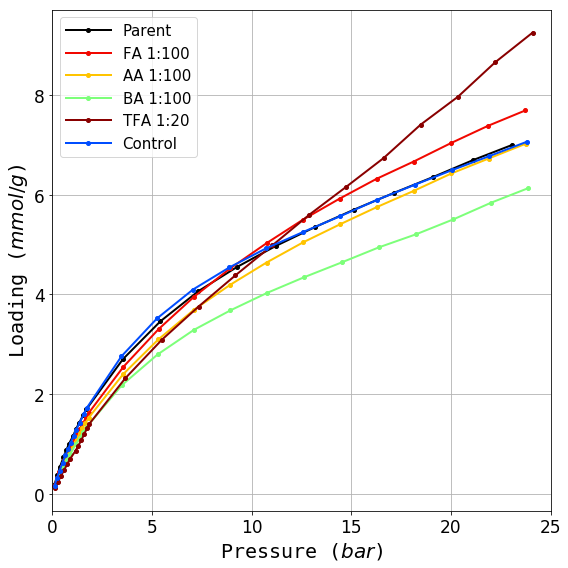
\includegraphics[width=\textwidth]{co2phys/co2-iso}%
		\caption{}%
		\label{def:fig:co2-iso-reg}
	\end{subfigure}%
	\begin{subfigure}{0.5\linewidth}
		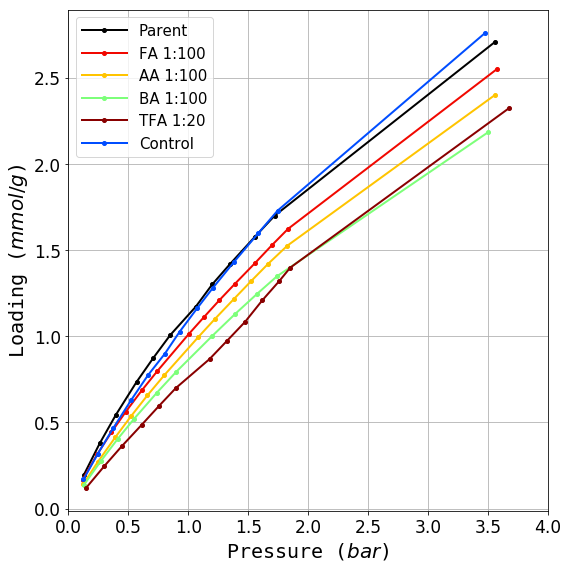
\includegraphics[width=\textwidth]{co2phys/co2-iso-log}%
		\caption{}%
		\label{def:fig:co2-iso-log}
	\end{subfigure}%

    \caption{
        \ce{CO2} adsorption isotherms at \SI{303}{\kelvin} on different
        materials leached in \gls{DMSO} in the (a) \SIrange{0}{25}{\bar} range
        and the (b) \SIrange{0}{4}{\bar} range. All materials were 
        activated at \SI{200}{\degreeCelsius}.
    }\label{def:fig:co2-iso}
\end{figure}

Isotherms follow similar trends as observed with nitrogen sorption and
\gls{TGA} analysis. A large increase in amount adsorbed can be
seen on the \gls{TFA} leached sample, with almost a doubling in the 
capacity at high pressure ranges. These values can only be obtained 
if a missing cluster \textit{reo} net is the dominant phase of the 
material. Combined with the increased interactions with the framework
at low loadings due to the fluorine moieties, this variant shows an
astounding increase in adsorption capacity.
The formate leached sample exhibits a cross-over of the parent 
material isotherm, highly similar to the simulated missing linker isotherms 
with around 11 linkers per metal node. A similar pattern may be 
present in the acetic acid isotherm, but with the intersection point
at around \SI{20}{\bar}. The benzoic acid isotherm
is shifted downwards throughout the entire pressure range, a further
indication that this modulator has a counterproductive effect for
obtaining defective materials through leaching.
Finally, the control and parent materials have nearly identical isotherms,
which confirms that the solvent does not act alone to generate 
defects in the structure.
